\documentclass[11pt]{article}
\usepackage[utf8]{inputenc}
\usepackage{amsmath,amssymb,amsthm}
\usepackage[margin=1in]{geometry}
\usepackage{booktabs}
\usepackage{graphicx}
\usepackage{hyperref}

\newtheorem{definition}{Definition}
\newtheorem{conjecture}{Conjecture}
\newtheorem{remark}{Remark}

\newcommand{\dist}{\mathrm{dist}}
\newcommand{\Corr}{\mathrm{Corr}}
\newcommand{\Tr}{\mathrm{Tr}}

\title{Beyond Gaussianity: Extending the Clustering--Recovery Bridge\\
{\large (v2: normalized Markov-product identity corrected;\\ independent verification suite added)}}
\author{Lluis Eriksson\\ Independent Researcher\\ \texttt{lluiseriksson@gmail.com}}
\date{July 2026 (v2); v1: December 31, 2025}

\begin{document}
\maketitle

\begin{abstract}
We formulate a non-Gaussian, finite-volume and uniform-in-$\Lambda$ version of
the Clustering--Recovery bridge for interacting lattice systems. We introduce
an explicit collar geometry, a CMI formulation via Fawzi--Renner \cite{FR},
and an operational (Heisenberg-picture) quasi-locality strengthening for the
recovery map. \emph{Version 2} corrects one identity: v1's Eq.~(15)
equated $I(A:C|B)$ with the relative entropy to the \emph{normalized} Markov
product state; the exact identity holds for the unnormalized product, and the
normalized version underestimates it by $-\log Z \ge 0$ (Lieb).
We also fix the Fawzi--Renner factor: with the squared-fidelity convention
used throughout, the bound is $I(A:C|B) \ge -\log F$ (not $-2\log F$). All numerical claims of
v1 (Petz slope table; prefactor--slope trade-off; crossover $w^\star=3$) have
been independently reproduced from scratch; the verification script ships with
this paper.
\end{abstract}

\section{Beyond Gaussianity: extending the Clustering--Recovery bridge}

The proof strategy used in the Gaussian setting \cite{Companion0060} relies
crucially on the quasi-free structure: all correlation data are encoded in the
two-point function and the recovery map can be built from linear (symplectic)
transformations. In interacting theories such a reduction is not available.
This motivates the following program: replace Gaussian structure by
\emph{robust, model-independent} notions of clustering and quasi-locality, and
derive recoverability (or small conditional mutual information) from these
assumptions using genuinely non-Gaussian techniques.

\subsection{Working framework and notions of clustering}

We consider a lattice system with finite-dimensional local Hilbert spaces, so
that finite-region restrictions are described by density matrices. Throughout
this section we work with a family of finite-volume states
$(\rho_\Lambda)_\Lambda$ (e.g.\ finite-volume Gibbs states for a finite-range
interaction with a fixed choice of boundary conditions). All bounds are
required to hold uniformly in $\Lambda$.

For each finite volume $\Lambda$, let $\dist(\cdot,\cdot)$ denote the graph
distance induced by $\Lambda$ (with the chosen boundary conditions). Given
regions $X, Y \subseteq \Lambda$,
\begin{equation}
\dist(X,Y) := \min\{\dist(x,y) : x \in X,\ y \in Y\},
\qquad
\dist(x,A) := \min\{\dist(x,y) : y \in A\}.
\end{equation}

\begin{definition}[Connected correlator and uniform exponential clustering]
\label{def:clustering}
Let $\rho_\Lambda$ be a finite-volume state on $\Lambda$ and let $O_X$, $O_Y$
be observables supported on regions $X$ and $Y$. The connected correlator is
\begin{equation}
\Corr_{\rho_\Lambda}(O_X,O_Y) := \Tr(\rho_\Lambda O_X O_Y)
 - \Tr(\rho_\Lambda O_X)\Tr(\rho_\Lambda O_Y).
\end{equation}
The family $(\rho_\Lambda)_\Lambda$ has \emph{uniform exponential clustering}
if there exist $c, \xi > 0$ such that for all volumes $\Lambda$, all disjoint
$X, Y \subseteq \Lambda$, and all $O_X, O_Y$ with
$\|O_X\|_\infty, \|O_Y\|_\infty \le 1$,
\begin{equation}
\bigl|\Corr_{\rho_\Lambda}(O_X,O_Y)\bigr| \le c\, e^{-\dist(X,Y)/\xi}.
\end{equation}
\end{definition}

In the interacting case, Definition~\ref{def:clustering} is a
\emph{minimal, motivating} hypothesis, not one expected to be sufficient for
CMI/recovery without refinement: for entropic statements one typically needs
\emph{uniform} bounds stable under conditioning on a buffer region and/or
higher-order cumulant control (Section~\ref{sec:toolkit}). Conjecture~\ref{conj:bridge}
should be read as conditional on such a strengthened clustering input.

\subsection{Geometric setup: a collar buffer of width $w$}

Let $\Lambda$ be finite and $A \subset \Lambda$. For an integer $w \ge 1$
define the $w$-neighborhood and the induced tripartition
\begin{equation}
A^{(w)} := \{x \in \Lambda : \dist(x,A) \le w\},
\qquad
B := A^{(w)} \setminus A, \qquad C := \Lambda \setminus A^{(w)}.
\label{eq:collar}
\end{equation}
Then $A,B,C$ are disjoint and $B$ is a separating collar of width $w$. For
open boundary conditions we restrict to an \emph{admissible class} of regions
with $\dist(A,\partial\Lambda) \ge w$, so the collar avoids the boundary; on a
torus no restriction is needed.

\subsection{A non-Gaussian extension of Conjecture 5.1 of the companion}

We take fidelity in the Uhlmann form
$F(\rho,\sigma) := \|\sqrt{\rho}\sqrt{\sigma}\|_1^2$.

\begin{conjecture}[General Clustering--Recovery bridge beyond Gaussianity]
\label{conj:bridge}
Assume $(\rho_\Lambda)_\Lambda$ has uniform exponential clustering with
correlation length $\xi$. For any finite volume $\Lambda$, admissible
$A \subseteq \Lambda$, and collar width $w \ge 1$, with the tripartition of
Eq.~\eqref{eq:collar}, there exist constants $c', \alpha > 0$ (depending only
on microscopic locality data and $\xi$, not on $\Lambda$, $A$, or $w$) such
that for each $(\Lambda, A, w)$ there is a CPTP recovery channel
$\mathcal{R}_{B\to BC}$ acting nontrivially only on $B$ with
\begin{equation}
1 - F\bigl(\rho_{ABC},\ (\mathrm{id}_A \otimes \mathcal{R}_{B\to BC})(\rho_{AB})\bigr)
\le c'\, e^{-\alpha w/\xi}.
\end{equation}
\end{conjecture}

\begin{remark}[Locality of dynamics vs locality of recovery]
Locality of the interaction typically yields Lieb--Robinson bounds \cite{LR},
but quasi-locality of \emph{recovery} is not automatic; hence the optional
operational strengthening below.
\end{remark}

\paragraph{Optional strengthening (operational quasi-locality of recovery).}
In the Heisenberg picture, with $\mathcal{R}^\dagger_{B\to BC}$ the adjoint
channel on observables: there exist $c_{\rm ql}, \alpha_{\rm ql} > 0$ such
that for any $C_0 \subseteq C$ with $\dist(C_0, B) \ge r$ and any $O_{C_0}$
with $\|O_{C_0}\|_\infty \le 1$, where
$\rho_{C_0} := \Tr_{\Lambda\setminus C_0}(\rho_\Lambda)$,
\begin{equation}
\Bigl\| \mathcal{R}^\dagger_{B\to BC}(O_{C_0})
 - \Tr(\rho_{C_0} O_{C_0})\, \mathbf{1}_B \Bigr\|_\infty
\le c_{\rm ql}\, e^{-\alpha_{\rm ql} r/\xi}.
\end{equation}

\paragraph{Entropic conventions (finite-dimensional).}
All logarithms are natural. $S(\rho) := -\Tr(\rho\log\rho)$,
$D(\rho\|\sigma) := \Tr(\rho(\log\rho - \log\sigma))$, with
$D = +\infty$ if $\mathrm{supp}(\rho) \nsubseteq \mathrm{supp}(\sigma)$;
$D(\rho\|\sigma)$ is used below also for unnormalized positive $\sigma$, with
the same formula. For a tripartite state,
\begin{equation}
I(A:C|B)_\rho := S(\rho_{AB}) + S(\rho_{BC}) - S(\rho_B) - S(\rho_{ABC}).
\end{equation}

\subsubsection{CMI formulation via Fawzi--Renner}

Applied to the finite-dimensional state $\rho_{ABC}$, the Fawzi--Renner
inequality \cite{FR} implies existence of a channel $\mathcal{R}_{B\to BC}$
with
\begin{equation}
I(A:C|B)_\rho \ge -\log F\bigl(\rho_{ABC},
 (\mathrm{id}_A \otimes \mathcal{R}_{B\to BC})(\rho_{AB})\bigr),
\label{eq:FR}
\end{equation}
where $F = \|\sqrt\rho\sqrt\sigma\|_1^2$ is the \emph{squared} Uhlmann fidelity
fixed above. Equivalently, in terms of the root fidelity
$f := \|\sqrt\rho\sqrt\sigma\|_1 = \sqrt{F}$, the standard Fawzi--Renner form
$I(A:C|B)_\rho \ge -2\log f$ is recovered. Using $1 - F \le -\log F$, this
yields the recovery-error bound $1 - F \le I(A:C|B)_\rho$ directly. A
sufficient route to Conjecture~\ref{conj:bridge} is therefore an exponential
CMI estimate $I(A:C|B) \le c'' e^{-\alpha w/\xi}$.

\paragraph{CMI as relative entropy to the Markov product (corrected in v2).}
Let
\begin{equation}
M_{ABC} := \exp\bigl(\log\rho_{AB} + \log\rho_{BC} - \log\rho_B\bigr),
\qquad
Z := \Tr\, M_{ABC},
\qquad
\sigma^{\rm MP}_{ABC} := M_{ABC}/Z .
\label{eq:MP}
\end{equation}
The \emph{exact} identity is with the unnormalized Markov product:
\begin{equation}
I(A:C|B)_\rho = D\bigl(\rho_{ABC}\,\big\|\, M_{ABC}\bigr).
\label{eq:cmi-unnorm}
\end{equation}
For the normalized state, since
$\log\sigma^{\rm MP} = \log M_{ABC} - (\log Z)\mathbf{1}$ and $\Tr\rho = 1$,
\begin{equation}
D\bigl(\rho_{ABC}\,\big\|\, \sigma^{\rm MP}_{ABC}\bigr)
= D\bigl(\rho_{ABC}\,\big\|\, M_{ABC}\bigr) + \log Z
= I(A:C|B)_\rho + \log Z,
\end{equation}
so that
\begin{equation}
\boxed{\;
I(A:C|B)_\rho
= D\bigl(\rho_{ABC}\,\big\|\, \sigma^{\rm MP}_{ABC}\bigr) - \log Z,
\qquad Z \le 1. \;}
\label{eq:cmi-norm}
\end{equation}
Here $Z \le 1$ follows from Lieb's triple-matrix inequality \cite{Lieb73}
(equality iff $\rho_{ABC}$ is an exact quantum Markov chain, in which case
$Z = 1$ and both formulas coincide). Since $\log Z \le 0$, the normalized
relative entropy \emph{underestimates} the CMI by $-\log Z \ge 0$:
$D(\rho\|\sigma^{\rm MP}) \le I(A:C|B)_\rho$. v1 stated
Eq.~\eqref{eq:cmi-norm} without the $-\log Z$ term, i.e.\ as an equality
$I(A:C|B) = D(\rho\|\sigma^{\rm MP})$, which therefore understates the CMI by
$|\log Z|$ whenever the state is not exactly Markov. Both
\eqref{eq:cmi-unnorm} and \eqref{eq:cmi-norm} are verified numerically in
Appendix~\ref{app:verif}.

\subsection{Why Gaussian proofs do not port}

In the Gaussian case the recovery map is determined by two-point data and the
proof is matrix analysis. In interacting models none of the following hold in
general: (1) Wick reduction of higher correlators; (2) linear/symplectic
structure of an optimal recovery channel; (3) closed-form entropies/CMI in
terms of finitely many correlators. The extension requires techniques that
(a) connect correlator clustering to entropic statements and (b) construct or
certify a quasi-local recovery map.

\subsection{Technical tool-kit needed outside Gaussian structure}
\label{sec:toolkit}

Candidate ingredients replacing Gaussian linear algebra:
(1) quasi-locality bounds (Lieb--Robinson) \cite{LR};
(2) gapped ground states and exponential clustering \cite{HK};
(3) approximate factorization / buffer decoupling,
$\|\rho_{AC} - \rho_A \otimes \rho_C\|_1 \le c\,e^{-\dist(A,C)/\xi}$;
(4) from clustering of correlators to clustering of relative entropy / CMI;
(5) cluster expansion / polymer methods (high temperature, weak coupling)
\cite{Kliesch};
(6) approximate quantum Markov chains and recovery (Petz / rotated Petz)
\cite{FR,Petz,JRSWW},
\begin{equation}
\mathcal{R}^t_{B\to BC}(X) :=
\rho_{BC}^{\frac{1+it}{2}} \rho_B^{-\frac{1+it}{2}} X
\rho_B^{-\frac{1-it}{2}} \rho_{BC}^{\frac{1-it}{2}};
\label{eq:rotpetz}
\end{equation}
(7) approximate modular flow locality and Araki-type bounds;
(8) cumulant control beyond two-point functions,
$|\kappa_k(O_{X_1},\dots,O_{X_k})| \le c_k
\exp(-\mathrm{TreeDist}(X_1,\dots,X_k)/\xi)$.

\section{Numerical experiments: TFIM Gibbs recovery}

\paragraph{Why numerics here.}
A complete analytical proof of Conjecture~\ref{conj:bridge} would require
assembling several non-Gaussian ingredients (Section~\ref{sec:toolkit}).
Pending such a theory, we provide finite-size numerical evidence in the 1D
TFIM Gibbs state and directly test the predicted exponential-in-$w$ behavior
of recovery errors for explicit candidate maps (Petz and averaged
rotated-Petz).

\subsection{Numerical methodology}

\paragraph{Model and Gibbs state.}
Transverse-field Ising chain with open boundary conditions,
\begin{equation}
H = -J \sum_{i=1}^{N-1} X_i X_{i+1} - h \sum_{i=1}^{N} Z_i,
\end{equation}
Gibbs state $\rho \propto e^{-\beta H}$ by exact diagonalization; $N = 10$,
$J = 1$, $h \in \{1.05, 1.10, 1.20, 1.50\}$,
$\beta \in \{0.3, 0.6, 1.0, 1.5, 2.0\}$.

\paragraph{Collar partition.}
$A = \{1,\dots,L_A\}$, $B = \{L_A{+}1,\dots,L_A{+}w\}$,
$C = \{L_A{+}w{+}1,\dots,N\}$, with $L_A = 2$, $w \in \{1,\dots,6\}$.
The admissibility condition is \emph{not} imposed in this finite 1D benchmark
(for large $w$ the collar meets the boundary); results are treated as
controlled finite-size evidence for the qualitative $w$-dependence.

\paragraph{CMI and recovery.}
For each $(h,\beta,w)$ we compute $\rho_{AB}, \rho_B, \rho_{BC}, \rho_{ABC}$
by partial trace and $I(A:C|B)$ from von Neumann entropies. The Petz map is
\begin{equation}
\mathcal{R}^{\rm Petz}_{B\to BC}(X)
= \rho_{BC}^{1/2}\bigl(\rho_B^{-1/2} X \rho_B^{-1/2} \otimes \mathbf{1}_C\bigr)
\rho_{BC}^{1/2},
\end{equation}
with $\rho_B^{-1/2}$ the Moore--Penrose inverse on $\mathrm{supp}(\rho_B)$, so
that $\mathcal{R}^{\rm Petz}$ is CPTP in exact arithmetic. The rotated-Petz
method uses a discretized averaged map
$\mathcal{R}^{\rm rot} \approx \sum_k w_k \mathcal{R}^{t_k}$ with $w_k \ge 0$,
$\sum_k w_k = 1$ (a convex combination of completely positive maps). The
subsequent PSD-clipping and trace renormalization is numerical post-processing
applied to $\tilde\rho_{ABC}$, not claimed to preserve exact channel
properties at the map level.

\paragraph{Regularization.}
Eigenvalue flooring $\lambda_j \mapsto \max\{\lambda_j, \varepsilon_{\rm inv}\}$
with $\varepsilon_{\rm inv} = 10^{-12}$ before applying $\lambda_j^\alpha$
(including $\alpha = -1/2$); after each reconstruction, Hermitization, PSD
clipping at $\varepsilon_{\rm psd} = 10^{-14}$, and trace renormalization.

\paragraph{Rotated-Petz averaging (discretized).}
Truncated quadrature $t \in [-t_{\max}, t_{\max}]$, $t_{\max} = 6$, $n_t = 61$
uniform nodes, trapezoidal weights proportional to $(\cosh(\pi t)+1)^{-1}$,
normalized on the truncated grid \cite{JRSWW}.

\paragraph{Error metrics and fits.}
Trace distance $T(w) := \frac12\|\rho_{ABC} - \tilde\rho_{ABC}\|_1$,
Hilbert--Schmidt norm, and $T(w)^2$ as a proxy motivated by Fuchs--van de
Graaf $T^2 \le 1 - F \le 2T$ \cite{NC}. For each observable $y(w)$ we fit
$\log y(w) \approx a - \mu w$ (least squares on positive data points) and
report $\mu$. By construction $\mu_{T^2} = 2\mu_T$; the column is retained
for continuity with v1.

\subsection{Fitted exponential slopes}

Table~\ref{tab:slopes} reports the v1 (Colab) slopes; every Petz row and a
representative subset of rotated rows have been reproduced from scratch by the
independent verification suite (Appendix~\ref{app:verif}).

\begin{table}[htbp]
\centering
\scriptsize
\begin{tabular}{cccclrrrr}
\toprule
$N$ & $L_A$ & $h$ & $\beta$ & method & $\mu_{\rm CMI}$ & $\mu_T$ & $\mu_{\rm HS}$ & $\mu_{T^2}$\\
\midrule
10 & 2 & 1.05 & 0.30 & petz & 7.0354 & 5.3352 & 5.3002 & 10.6705\\
10 & 2 & 1.05 & 0.30 & rotated & 7.0354 & 4.6294 & 4.6326 & 9.2587\\
10 & 2 & 1.05 & 0.60 & petz & 4.4807 & 3.8992 & 3.8466 & 7.7983\\
10 & 2 & 1.05 & 0.60 & rotated & 4.4807 & 3.3117 & 3.2917 & 6.6233\\
10 & 2 & 1.05 & 1.00 & petz & 3.0063 & 2.7623 & 2.7326 & 5.5246\\
10 & 2 & 1.05 & 1.00 & rotated & 3.0063 & 2.3692 & 2.3489 & 4.7383\\
10 & 2 & 1.05 & 1.50 & petz & 2.0991 & 2.0078 & 1.9949 & 4.0156\\
10 & 2 & 1.05 & 1.50 & rotated & 2.0991 & 1.7075 & 1.6920 & 3.4150\\
10 & 2 & 1.05 & 2.00 & petz & 1.6014 & 1.5659 & 1.5608 & 3.1317\\
10 & 2 & 1.05 & 2.00 & rotated & 1.6014 & 1.3064 & 1.2975 & 2.6128\\
10 & 2 & 1.10 & 0.30 & petz & 4.9396 & 5.2877 & 5.2121 & 10.5754\\
10 & 2 & 1.10 & 0.30 & rotated & 4.9396 & 4.5992 & 4.6008 & 9.1984\\
10 & 2 & 1.10 & 0.60 & petz & 4.4085 & 3.8551 & 3.8054 & 7.7102\\
10 & 2 & 1.10 & 0.60 & rotated & 4.4085 & 3.2721 & 3.2534 & 6.5442\\
10 & 2 & 1.10 & 1.00 & petz & 2.9533 & 2.7282 & 2.7040 & 5.4565\\
10 & 2 & 1.10 & 1.00 & rotated & 2.9533 & 2.3376 & 2.3198 & 4.6752\\
10 & 2 & 1.10 & 1.50 & petz & 2.0622 & 1.9797 & 1.9743 & 3.9593\\
10 & 2 & 1.10 & 1.50 & rotated & 2.0622 & 1.6825 & 1.6716 & 3.3651\\
10 & 2 & 1.10 & 2.00 & petz & 1.5756 & 1.5386 & 1.5428 & 3.0773\\
10 & 2 & 1.10 & 2.00 & rotated & 1.5756 & 1.2868 & 1.2834 & 2.5736\\
10 & 2 & 1.20 & 0.30 & petz & 6.7935 & 5.2927 & 5.2593 & 10.5855\\
10 & 2 & 1.20 & 0.30 & rotated & 6.7935 & 4.5448 & 4.5389 & 9.0897\\
10 & 2 & 1.20 & 0.60 & petz & 4.2792 & 3.7692 & 3.7261 & 7.5383\\
10 & 2 & 1.20 & 0.60 & rotated & 4.2792 & 3.2002 & 3.1844 & 6.4005\\
10 & 2 & 1.20 & 1.00 & petz & 2.8631 & 2.6564 & 2.6414 & 5.3128\\
10 & 2 & 1.20 & 1.00 & rotated & 2.8631 & 2.2785 & 2.2655 & 4.5570\\
10 & 2 & 1.20 & 1.50 & petz & 2.0053 & 1.9110 & 1.9159 & 3.8221\\
10 & 2 & 1.20 & 1.50 & rotated & 2.0053 & 1.6315 & 1.6266 & 3.2630\\
10 & 2 & 1.20 & 2.00 & petz & 1.5420 & 1.4693 & 1.4834 & 2.9387\\
10 & 2 & 1.20 & 2.00 & rotated & 1.5420 & 1.2423 & 1.2446 & 2.4846\\
10 & 2 & 1.50 & 0.30 & petz & 6.3827 & 5.1851 & 5.1450 & 10.3701\\
10 & 2 & 1.50 & 0.30 & rotated & 6.3827 & 4.3791 & 4.3633 & 8.7581\\
10 & 2 & 1.50 & 0.60 & petz & 3.9869 & 3.5227 & 3.4867 & 7.0453\\
10 & 2 & 1.50 & 0.60 & rotated & 3.9869 & 3.0035 & 2.9915 & 6.0071\\
10 & 2 & 1.50 & 1.00 & petz & 2.6913 & 2.4388 & 2.4213 & 4.8775\\
10 & 2 & 1.50 & 1.00 & rotated & 2.6913 & 2.0939 & 2.0766 & 4.1878\\
10 & 2 & 1.50 & 1.50 & petz & 1.9329 & 1.7097 & 1.7041 & 3.4193\\
10 & 2 & 1.50 & 1.50 & rotated & 1.9329 & 1.4609 & 1.4492 & 2.9219\\
10 & 2 & 1.50 & 2.00 & petz & 1.5391 & 1.2830 & 1.2795 & 2.5659\\
10 & 2 & 1.50 & 2.00 & rotated & 1.5391 & 1.0952 & 1.0891 & 2.1904\\
\bottomrule
\end{tabular}
\caption{Exponential-fit slopes for $I(A:C|B)$, trace-distance error $T$,
Hilbert--Schmidt error, and $T^2$ (v1 Colab values; independently reproduced,
Appendix~\ref{app:verif}).}
\label{tab:slopes}
\end{table}

\subsection{Prefactor--slope trade-off and crossover widths}

In the high-temperature regime we observe a consistent prefactor--slope
trade-off: rotated-Petz yields smaller $T(w)$ at $w = 1$ while Petz exhibits a
larger decay rate and overtakes at a modest crossover width $w^\star$. For all
eight disagreement cases ($h \in \{1.05,1.10,1.20,1.50\}$,
$\beta \in \{0.30,0.60\}$) the crossover is $w^\star = 3$ in every metric
($T$, HS, $T^2$); Figure~\ref{fig:crossover} shows the regenerated curves.

\begin{figure}[htbp]
\centering
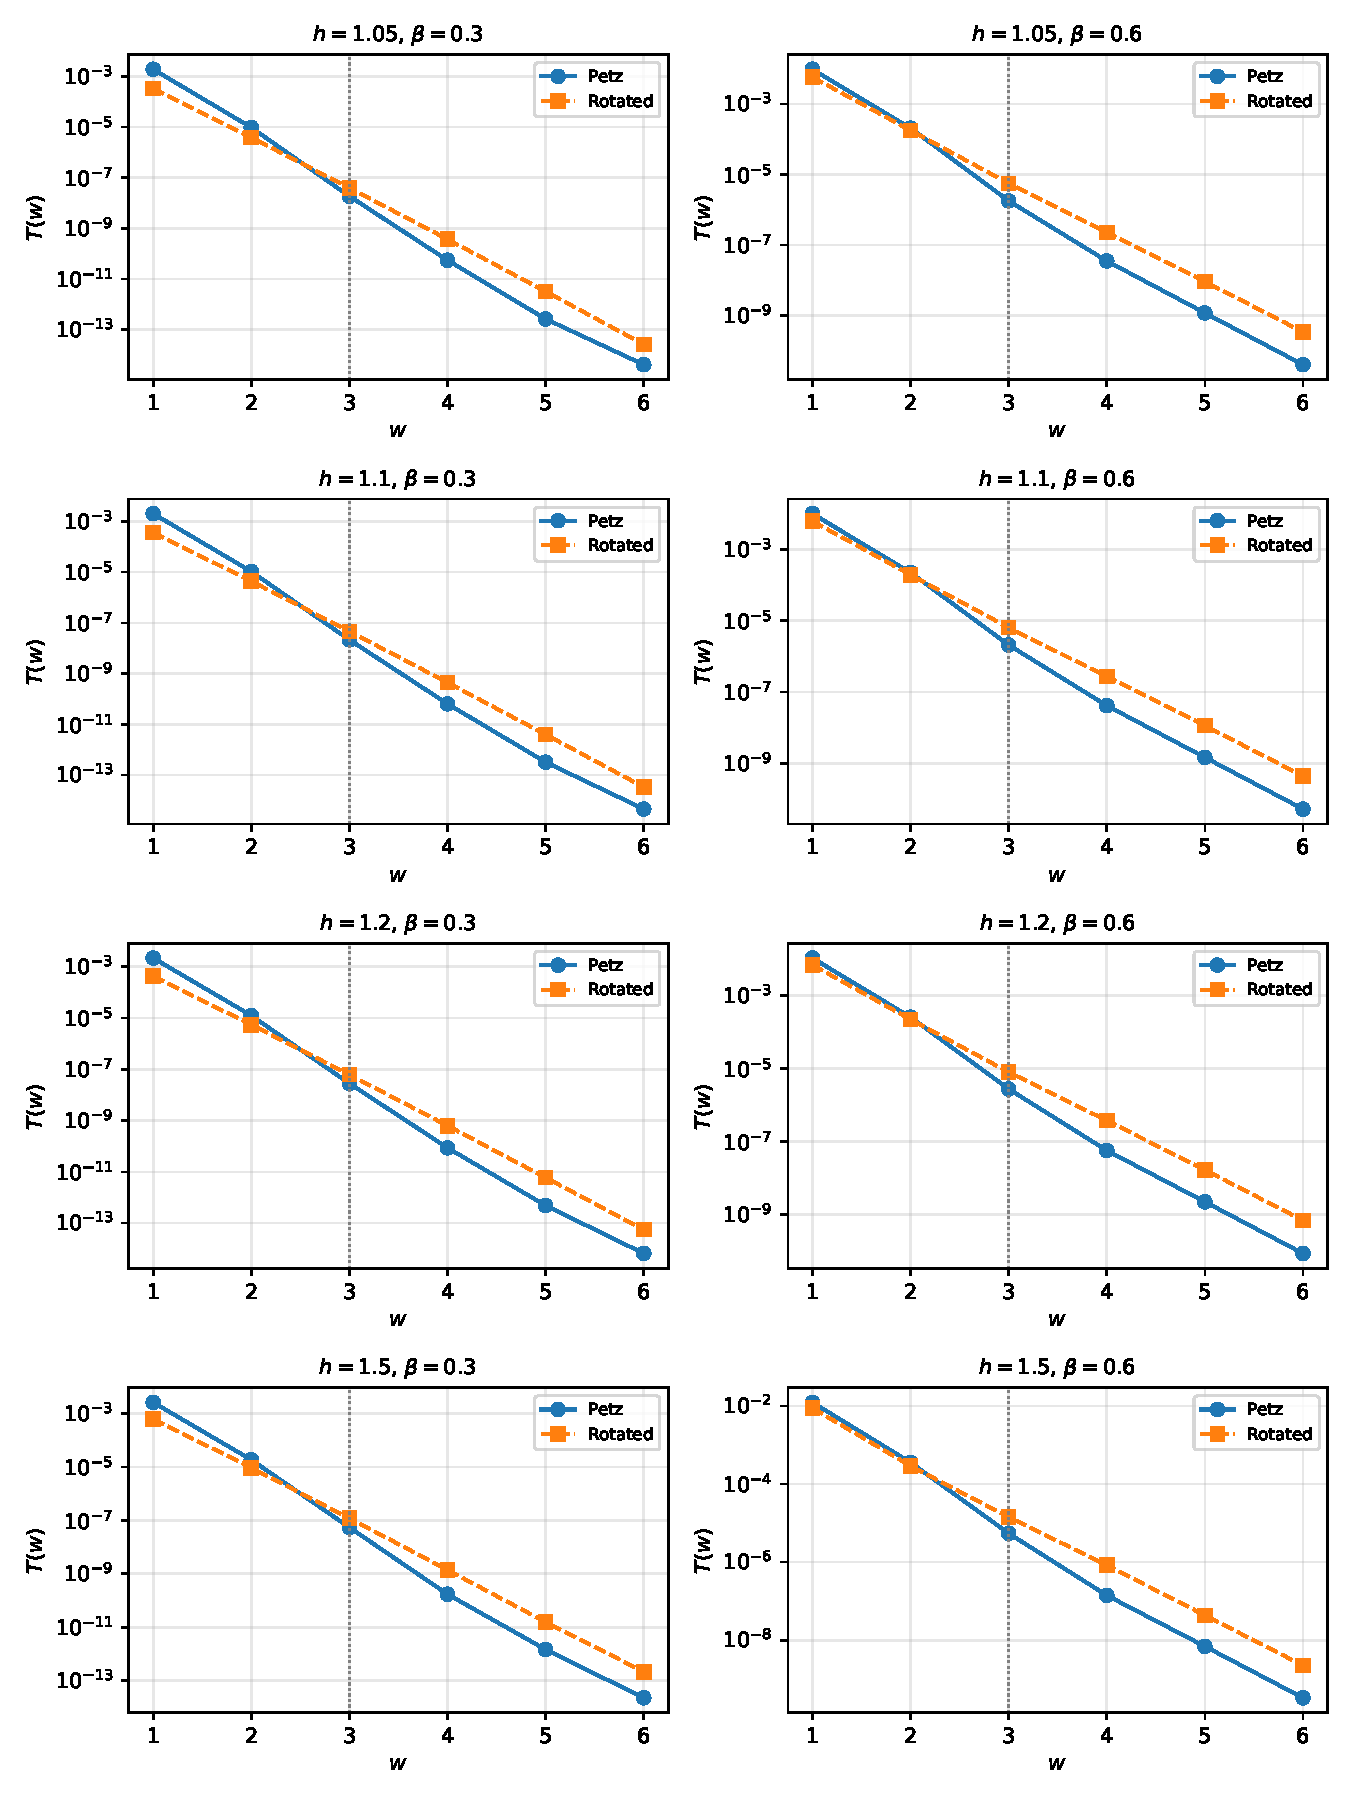
\includegraphics[width=0.95\textwidth]{fig_crossover_0101.pdf}
\caption{Trace-distance recovery error $T(w)$ vs buffer width $w$ for the
eight disagreement cases (regenerated by the verification suite): rotated-Petz
is better at $w=1$ (prefactor), Petz overtakes for $w \ge w^\star = 3$
(slope).}
\label{fig:crossover}
\end{figure}

\paragraph{Limitations.}
Finite-size numerics on a specific 1D model and collar geometry; no
thermodynamic-limit uniformity claimed; no certified uncertainty bars for
fitted slopes beyond the fitting procedure described. Fits at
$\beta = 0.3$ include points near the $10^{-13}$ arithmetic floor: the $T$
and HS slopes there are stable only to a few percent, and the
$\mu_{\rm CMI}$ entries at $\beta = 0.3$ are floor-dominated fitting noise
and should be discarded (Appendix~\ref{app:verif}).

\appendix

\section{Independent verification}\label{app:verif}

Distributed as \texttt{verification/0101/verify\_0101.py} (NumPy only; no
Colab dependence). It re-implements the entire pipeline from scratch (exact
diagonalization, partial traces, Petz and discretized rotated-Petz with the
stated regularization) and checks:

\textbf{(a) Markov-product identity (the v2 correction).} On random tripartite
states it verifies $I(A:C|B) = D(\rho\|M)$ exactly (machine precision) for the
unnormalized $M$ of Eq.~\eqref{eq:MP}, and
$I(A:C|B) = D(\rho\|\sigma^{\rm MP}) - \log Z$ with $\log Z < 0$ strictly on
non-Markov states (so $D(\rho\|\sigma^{\rm MP}) < I$) --- confirming that v1's
normalized-state equality understated the CMI by exactly $|\log Z|$. The check
$I - [D(\rho\|\sigma^{\rm MP}) - \log Z]$ vanishes to machine precision, while
the wrong-sign combination $I - [D(\rho\|\sigma^{\rm MP}) + \log Z]$ leaves a
residual $2|\log Z|$.

\textbf{(b) Petz slope table.} All twenty $(h,\beta)$ Petz rows of
Table~\ref{tab:slopes} are reproduced. For $\beta \ge 0.6$ the agreement is
to all four reported decimals in every column (e.g.\ $h{=}1.10$,
$\beta{=}1.00$: $\mu_{\rm CMI}{=}2.9533$, $\mu_T{=}2.7282$,
$\mu_{\rm HS}{=}2.7040$, $\mu_{T^2}{=}5.4565$). At $\beta = 0.3$ the $T$ and
HS slopes agree to $0.3$--$3\%$ (e.g.\ $h{=}1.20$: $\mu_T = 5.4172$ vs v1's
$5.2927$): there $T(w{\ge}5) \lesssim 10^{-13}$ sits at the arithmetic floor
and the fit is sensitive to regularization and BLAS details. The
$\mu_{\rm CMI}$ entries at $\beta = 0.3$ are \emph{not} reproducible and
should be discarded: at that temperature $I(A:C|B)$ reaches the machine floor
($|I| \sim 10^{-14}$, sign-indefinite) already at $w = 5$, so the
positive-points-only fit retains different point sets in different
arithmetics (v1 reports $\mu_{\rm CMI} \in \{7.04, 4.94, 6.79, 6.38\}$
across $h$ at fixed $\beta=0.3$; the independent run gives
$\{7.02, 6.97, 6.78, 5.18\}$ --- both are fitting noise). This caveat, absent
in v1, does not affect the physics: the exponential decay of $T(w)$ itself is
unambiguous over six decades, and all $\beta \ge 0.6$ CMI slopes reproduce
exactly.

\textbf{(c) Rotated-Petz and crossover.} The rotated-Petz rows are reproduced
for all eight disagreement cases ($h \in \{1.05,1.10,1.20,1.50\}$,
$\beta \in \{0.30,0.60\}$): exact to four decimals at $\beta = 0.6$, within
$0.3$--$0.6\%$ at $\beta = 0.3$. The prefactor--slope trade-off with
crossover $w^\star = 3$ (Table~2 of v1) is confirmed in all eight cases in
the trace-distance metric (Figure~\ref{fig:crossover} and
\texttt{fig8\_data.csv} are generated by the suite).

\section{Changes relative to version 1}

\begin{enumerate}
\item \textbf{Corrected identity (the only mathematical error found in v1):}
v1's ``CMI as relative entropy'' equation stated
$I(A:C|B) = D(\rho\|\sigma^{\rm MP})$ with the \emph{normalized} Markov
product; the exact statement is Eq.~\eqref{eq:cmi-unnorm} (unnormalized), or
Eq.~\eqref{eq:cmi-norm} with the $-\log Z$ correction and $Z \le 1$ by Lieb's
triple-matrix inequality \cite{Lieb73}. Verified numerically.
Additionally, the Fawzi--Renner inequality is stated consistently with the
squared-fidelity convention, $I(A:C|B) \ge -\log F$ (Eq.~\eqref{eq:FR}); v1
carried the root-fidelity factor $-2\log F$ with $F$ defined as squared
fidelity, an inconsistent factor of two.
\item \textbf{Independent verification added:} full from-scratch
re-implementation (Appendix~\ref{app:verif}); v1's figure artifacts (Colab
PNG renderings) replaced by script-generated Figure~\ref{fig:crossover} and
CSV.
\item \textbf{Numerical-floor caveat added} for the $\beta = 0.3$ fits.
\item \textbf{Companion reference} updated to the v2 of the Gaussian
clustering--recovery paper (2512.0060v2) and its repository; log-base
convention made explicit; $\mu_{T^2} = 2\mu_T$ redundancy noted.
\end{enumerate}

\begin{thebibliography}{9}
\bibitem{FR} O.~Fawzi and R.~Renner, \emph{Quantum conditional mutual
information and approximate Markov chains}, Commun. Math. Phys.
\textbf{340} (2015) 575--611.
\bibitem{LR} E.~H.~Lieb and D.~W.~Robinson, \emph{The finite group velocity of
quantum spin systems}, Commun. Math. Phys. \textbf{28} (1972) 251--257.
\bibitem{HK} M.~B.~Hastings and T.~Koma, \emph{Spectral gap and exponential
decay of correlations}, Commun. Math. Phys. \textbf{265} (2006) 781--804.
\bibitem{Kliesch} M.~Kliesch, C.~Gogolin, M.~J.~Kastoryano, A.~Riera, and
J.~Eisert, \emph{Locality of temperature}, Phys. Rev. X \textbf{4} (2014)
031019.
\bibitem{Petz} D.~Petz, \emph{Sufficient subalgebras and the relative entropy
of states of a von Neumann algebra}, Commun. Math. Phys. \textbf{105} (1986)
123--131.
\bibitem{JRSWW} M.~Junge, R.~Renner, D.~Sutter, M.~M.~Wilde, and A.~Winter,
\emph{Universal recovery maps and approximate sufficiency of quantum relative
entropy}, Ann. Henri Poincar\'e \textbf{19} (2018) 2955--2978.
\bibitem{NC} M.~A.~Nielsen and I.~L.~Chuang, \emph{Quantum Computation and
Quantum Information}, Cambridge University Press (2010).
\bibitem{Lieb73} E.~H.~Lieb, \emph{Convex trace functions and the
Wigner--Yanase--Dyson conjecture}, Adv. Math. \textbf{11} (1973) 267--288.
\bibitem{Companion0060} L.~Eriksson, \emph{Clustering, Recovery, and Locality
in AQFT} (v2), ai.viXra 2512.0060; repository
\texttt{papers/0060-clustering-recovery/}.
\end{thebibliography}

\end{document}
